% !TEX encoding = UTF-8 Unicode

\documentclass[a4paper]{article}

\usepackage{color}
\usepackage{url}
\usepackage[T2A]{fontenc} % enable Cyrillic fonts
\usepackage[utf8]{inputenc} % make weird characters work
\usepackage{graphicx}
\graphicspath{ {img/} }

\usepackage[english,serbian]{babel}
%\usepackage[english,serbianc]{babel} %ukljuciti babel sa ovim opcijama, umesto gornjim, ukoliko se koristi cirilica

\usepackage[unicode]{hyperref}
\hypersetup{colorlinks,citecolor=green,filecolor=green,linkcolor=blue,urlcolor=blue}

%\newtheorem{primer}{Пример}[section] %ćirilični primer
\newtheorem{primer}{Primer}[section]

\begin{document}

%\renewcommand{\abstractname}{Apstrakt} %pisace Sazetak ako se ne ukljuci ova naredba

\title{Primena mašinskog učenja u verifikaciji softvera\\ \small{Seminarski rad u okviru kursa\\Metodologija stručnog i naučnog rada\\ Matematički fakultet}}

\author{Nikola Dimitrijević, Rastko Đorđević,\\
 Luka Živanović, Dimitrije Špadijer\\
 nikoladim95@gmail.com, mi14078@alas.matf.bg.ac.rs,\\
  mi14164@alas.matf.bg.ac.rs, mm11021@alas.matf.bg.ac.rs}
%\date{9.~april 2015.}
\vspace*{-3cm}
    {\let\newpage\relax\maketitle}

\abstract{
U ovom tekstu je ukratko prikazana osnovna forma seminarskog rada. Obratite pažnju da je pored ove .pdf datoteke, u prilogu i odgovarajuća .tex datoteka, kao i .bib datoteka korišćena za generisanje literature. Na prvoj strani seminarskog rada su naslov, apstrakt i sadržaj, i to sve mora da stane na prvu stranu! Kako bi Vaš seminarski zadovoljio standarde i očekivanja, koristite uputstva i materijale sa predavanja na temu pisanja seminarskih radova. Ovo je samo šablon koji se odnosi na fizički izgled seminarskog rada (šablon koji \emph{morate} da ispoštujete!) kao i par tehničkih pomoćnih uputstava. Molim Vas da kada budete predavali seminarski rad, imenujete datoteke tako da sadrže temu seminarskog rada, kao i imena i prezimena članova grupe (ili samo temu i prezimena, ukoliko je sa imenima predugačko). Predaja seminarskih radova biće isključivo preko web forme, a NE slanjem mejla.}

\tableofcontents

\newpage



% ==============================================================================
\section{Uvod}
\label{sec:uvod}
% ==============================================================================



Računarska rešenja se koriste za svemirske rakete, medicinsku opremu, samovozeće automobile i razne druge oblasti.
Sve veća zastupljenost i složenost softvera dovodi do veće verovatnoće katastrofalnog ishoda u slučaju greške.
Privremena nedostupnost vlastitog novca, pad satelita, prekomerno doziranje terapije pacijentima i puštanje nasilnih zatvorenika
na slobodu su primeri stvarnih događaja usled grešaka u programima.
Verifikacija softvera je oblast računarstva koja se bavi analizom softvera i ispitivanjem ispravnosti
programskog koda. Postoje razni alati za verifikaciju koji se uspešno koriste, ali postoje i mnoga ograničenja
u procesu analize koda koje je teško, a neke čak i nemoguće prevazići.
Analiziranje programskog koda se zasniva na formalnim matematičkim modelima koje je teško automatizovati.
Mašinsko učenje je postalo vrlo popularno i to sa pravom jer ima velike uspehe u raznim domenima,
pa je i prirodno nalaziti primene u okviru verifikacije softvera. Ovaj rad se nastavlja na \cite{micovic}
pa ovde neće biti prikazane već pomenute primene algoritama. U nastavku je dat opis verifikacije softvera,
modela mašinskog učenja koji su dalje korišćeni u razmatranim radovima, i konačno pregled konkretnih
primena mašinskog učenja kako u statičkoj tako i u dinamičkoj verifikaciji softvera.



% ==============================================================================
\section{Verifikacija softvera}
\label{sec:verifikacija}
% ==============================================================================



\par U savremenom dobu, računari i računarski sistemi predstavlju sastavni deo svakodnevice, kako u privatnom životu, tako i u poslovnom svetu, a i u državnoj administraciji. Zato je od izuzetnog značaja da softver koji se koristi bude pouzdan. Neispravan softver, u zavisnosti od toga gde se koristio i koliko je veliki bio propust, može izazvati male, ali i ogromne probleme sa teškim posledicama (čak i smrtnim). Oblast razvoja softvera koja se bavi proverom ispravnosti softvera, odnosno potvrđivanjem da softver radi u skladu sa zahtevima, naziva se \emph{verifikacija softvera}.

\par Potrebno je precizirati šta se podrazumeva pod ispravnim softverom. Razlikuju se pojmovi potpuno ispravnog i delimično ispravnog softvera. Softver se smatra potpuno ispravnim ako se zaustavlja za svaki ulaz i na izlazu daje ispravan rezultat, dok se delimično ispravnim softverom smatra onaj koji za ulaz daje ispravan rezultat ako se zaustavlja, a dozvoljeno je da se za neki ulaz program ne zaustavlja. Ne postoji algoritamski način da se proveri da li se neki program zaustavlja (tzv. Halting problem), pa se često ni ne ispituje potpuna, već samo delimična ispravnost softvera.

\par Postoje dve osnovne vrste verifikacije softvera. To su dinamička i statička verifikacija softvera.

\subsection{Dinamička verifikacija softvera}
\label{subsec:dinamicka}

\par Dinamička verifikacija softvera zasnovana je na tome da se provera ispravnosti softvera vrši tokom njegovog izvršavanja. Najčešće se dinamička verifikacija softvera vrši testiranjem i ti pojmovi se poistovećuju, što nije sasvim ispravno.

\par Testiranje je složen proces koji obuhvata pronalaženje što raznovrsnijeg skupa ulaza, definisanje očekivanih izlaza za svaki od tih ulaza, a zatim izvršavanje programa i provera da li je program za date ulaze vratio odgovarajuće izlaze. Postoje razne vrste i nivoi testova (da li imamo pristup izvornom kodu softvera ili ne, kao i da li testiramo jednu jedinicu koda ili više njih ili testiramo neku funkcionalnost softvera).

\par Testiranje služi da nam, u slučaju kada postoji greška u izvornom kodu softvera, ukaže na njeno postojanje. U zavisnosti od vrste testa, kao i nivoa, može se otkriti gde se u kodu nalazi greška, ali to često nije slučaj. Umesto toga, testovi samo otkrivaju postojanje grešaka.

\par Važno je imati na umu da testovi mogu dokazati isključivo neispravnost softvera, ali ne i njegovu (delimičnu) ispravnost. Da bi testiranje moglo dokazati delimičnu ili potpunu ispravnost softvera, neophodno bi bilo da skup ulaza bude jednak skupu svih teoretski dozvoljenih ulaza, a to, naravno, nije moguće, jer je taj skup beskonačan. Postavlja se pitanje zašto se onda uopšte testira. Odgovor je zato što se pažljivim odabirom skupa ulaza za koji će biti testirana ispravnost izlaza ne samo otklanjaju postojeće greške, nego i stiče sigurnost, odnosno poverenje u sam softver, tj. očekuje se da će broj neotkrivenih grešaka biti zanemarljiv.

\par Kao što je rečeno, često se dinamička verifikacija softvera poistovećuje sa testiranjem, iako je testiranje samo jedan od metoda. Pored testiranja postoji i debagovanje i ono očigledno spada u vid dinamičke verifikacije softvera. Naime, debagovanjem se može prekinuti rad programa u bilo kom trenutku i utvrditi trenutno stanje programa, a samim tim i potencijalno postojanje greške. Za razliku od testiranja koje se može vršiti i bez posedovanja izvornog koda softvera, debagovanje se vrši isključivo uz posedovanje koda, a često se može pronaći i tačno mesto na kome se nalazi greška.

\subsection{Statička verifikacija softvera}
\label{subsec:staticka}

\par Za razliku od dinamičke verifikacije softvera, \textit{statička verifikacija} podrazumeva analizu ispravnosti softvera bez njegovog pokretanja. Osnovna podela statičke verifikacije je na \textit{pregled koda (engl. code review)} i na \textit{automatizovanu verifikaciju}, koja će biti ključna za ostatak rada i biće podrazumevana kada se navodi pojam statička verifikacija.

\par Kao što je već pomenuto, ne postoji način da se za svaki program utvrdi da li se on zaustavlja ili ne, tako da nam i statička verifikacija ne može uvek dati željeni odgovor. Ipak, statička verifikacija može da nam da uvid u kvalitet koda i njegove propuste za mnoge netrivijalne probleme i zbog toga se razvijaju tehnike kojim bi skup takvih problema rastao, a vreme obrade se smanjivalo. 
\\\\

Neke od bitnijih tehnika statičke verifikacije su:
\begin{itemize}
\item \textbf{Analiza toka podataka} (engl. data flow analysis)
\item \textbf{Apstraktna interpretacija} (engl. abstract interpretation)
\item \textbf{Simbolička analiza} (engl. symbolic analysis)
\item \textbf{Proveravanje ograničenih modela} (engl. Bounded model checking), koja se najviše koristi za verifikaciju logičkih kola.
\end{itemize}

% TODO opisati tehnike koje smo koristili dole

% ==============================================================================
\section{Mašinsko učenje}
% ==============================================================================



\textit{Mašinsko učenje} bavi se proučavanjem indukcije, odnosno generalizacije 
čime formalizuje uopštavanje od uzorka određene veličine ka univerzalnim zaključcima. 
U srcu novog zamaha veštačke inteligencije nalazi se oblast mašinskog učenja. 
U nekim domenima, kao na primer prepoznavanje lica, u kojima se računari nisu 
mogli porediti sa ljudima po uspešnosti, ova oblast postiže rezultate superiorne 
u odnosu na rezultate ljudskih eksperata.

% TODO mozda ubaciti ovo, izbaciti nesto drugo
% Mašinsko učenje predstavlja automatsku detekciju smislenih šablona u podacima.

Mašinsko učenje je posebno pogodno za probleme koje je čoveku teško definisati a 
izuzetno lako za rešiti i u kojima je prihvatljiva poneka greška. Zbog dopuštanja 
povremenih greški u izvršavanju, ova oblast na prvi pogled izgleda kao nepogodna 
za rešavanje problema statičke verifikacije softvera. Ipak u stanju je da doprinese 
kao dodatni alat za rešavanje raznih problema koji se mogu naći u statičkoj 
verifikaciji ako njime rukuje prava osoba, čak i ako ne može da obeća kompletno 
rešenje svih problema.

Obično se identifikuju dve oblasti mašinskog učenja: \textit{nadgledano učenje} i 
\textit{nenadgledano učenje}. Nadgledano učenje odlikuje da pored ulaznih podataka 
postoji i njemu odgovarajući željeni izlaz. Model je zadužen za učenje pravila nad 
datim parovima ulaza i izlaza. Sa druge strane, kod nenadgledanog učenja dati su 
samo ulazni podaci pri čemu na algoritmu ostaje da pronađe strukturu u podacima. 

% TODO da li je naredna recenica suvisna
Za oblast statičke verifikacije najrelevantniji su algoritmi nadgledanog učenja, 
tako da će u ostatku rada biti predstavljeni isključivo algoritmi koji pripadaju toj oblasti.

Uobičajeni tok uspešne primene tehnika mašinskog učenja je sledeći. Nakon što se 
problem analizira, kao i podaci nad kojim će tehnike biti primenjene, potrebno je 
izabrati odgovarajući model. Nakon odabira modela, podaci se pretprocesiraju i 
izabrani model se trenira nad tako obrađenim podacima. Istrenirani model je dalje 
neophodno evaluirati kako bi bilo moguće znati u kojoj meri je koristan.

\subsection{Odabrani algoritmi}



\subsection{Evaluacija modela i mere kvaliteta}

%TODO da li je naredna rečenica suvišna?
Ukratko će biti predstavljeni termini vezani za \textit{meru kvaliteta} modela, 
kako bi bilo olakšano razumevanje postignutih rezultata u ostatku rada.

\textit{Evaluacija modela} predstavlja numeričko predstavljanje sposobnosti 
predviđanja datog modela na određenoj skali i direktno se oslanja na mere 
kvaliteta. Mere koje se najčešće sreću u klasifikaciji su \textit{tačnost}, 
\textit{preciznost}, \textit{odziv} i \textit{F1 mera}. Sve navedene mere 
izvedene su iz \textit{matrice konfuzije} \ref{table:matrica_konfuzije}.

\begin{table}[h]
	\centering
	\begin{tabular}{ |c|cc| } 
		\hline
		Stvarno / Predviđeno & Pozitivno & Negativno \\ 
		\hline
		Pozitivno & Stvarno Pozitivno & Lažno Negativno \\ 
		Negativno & Lažno Pozitivno & Stvarno Negativno \\ 
		\hline
	\end{tabular}
	\caption{Matrica konfuzije}
	\label{table:matrica_konfuzije}
	%\caption{ tabelica stagod}
\end{table}

Stvarno pozitivne i stvarno negativne instance su one instance koje su ispravno 
određene od strane modela. Lažno pozitivne instance su negativne instance za koje 
je od strane modela predviđeno da su pozitivne, dok su lažno negativne instance 
zapravo pozitivne instance koje je model loše klasifikovao kao negativne. 

% TODO dodati šta koje mere zapravo rade, zašto tačnost nije savršena, napomenuti da ima još raznih
Tačnost klasifikacije predstavlja procenat uspešno klasifikovanih instanci u odnosu 
na ukupan broj instanci. Preciznost je udeo ispravno pronađenih pozitivnih instanci 
u svim instancama koje su proglašene za pozitivne. Odziv je udeo ispravno pronađenih 
pozitivnih instanci u svim zaista pozitivnim instancama. Preciznost i odziv su dve 
mere koje najviše ima smisla razmatrati zajedno i način na koji se to najčešće radi 
je F1 mera, koja predstavlja njihovu harmonijsku sredinu.



% ==============================================================================
\section{Odabrani problemi statičke verifikacije}
\label{sec:naslovN}
% ==============================================================================



% TODO srediti ovo, odgovoriti na postavljena pitanja, dopuniti nakon što odlučimo šta će biti sva 4 problema
Predlozi za ovaj deo:

Kratak opis problema sa kojima ćemo se susreti u narednom delu poglavlja. 

Zašto su odabrani baš ovi problemi?

Predstojeći problemi su uređeni po uticaju koji su imali na oblast statičke verifikacije softvera.

Predlozi za dodatne baljezgarije kojima je mesto u ovom kutku rada su dobrodošli.


\subsection{Od izvornog koda do istreniranih modela}
\label{subsec:pregled}

Rad \cite{staticFeatures} predlaže rešenje za generisanje ulaznih podataka za algoritme mašinskog učenja na osnovu
izvornog koda kako bi se napravio inteligentni metod detekcije grešaka.

Bitno je prvo definisati kakvim tipovima grešaka se posvećuje pažnja u okviru metoda.
Iako postoje drukčije greške selekcija je vršena prema važnosti, odnosno prema tome
koliku štetu mogu da uzrokuju i mogućnost da budu detektovane računarskim alatom. Izabrani tipovi grešaka su:
% može se navesti iz koje knjige su uzete !!!!

\begin{itemize}
\item Prekoračenje bafera

\item Upravljanje memorijom

\item Dereferenciranje Null pokazivača

\item Kontrola toka

\item Konverzija označene celobrojne vrednosti u neoznačenu
\end{itemize}


Korišćen je WEKA softver koji je kolekcija algoritama mašinskog učenja.

Bogat skup funkcionalnosti koje pruža WEKA uključuje:
%lista
\begin{itemize}
\item Pretprocesiranje podataka i vizuelizacija
\item Selekcija atributa
\item Algoritmi klasifikacije
\item Algoritmi predviđanja
\item Algoritmi klasterovanja
\item Pravila asocijacije
\item Tehnike evaluacije
\end{itemize}


Za dati problem su najbitniji selekcija atributa i razni algoritmi klasifikacije i predviđanja.

Prvi prikazuju koji od brojnih elemenata ulaznog vektora su zapravo uključeni u proces donošenja odluke a koji nisu, dok
drugi klasifikuju odnosno predviđaju ispravnost na osnovu ulaza.
Međutim, najbitnija prednost koju pruža WAKA u odnosu na ostale dostupne alate je mogućnost da se koristi
jedan standardizovani format ulaza za sve raspoložive algoritme učenja što omogućava da se koristi jedan ulaz kako bi se isprobale
razne mogućnosti. Ulaz koji koristi WAKA je u formatu ARFF.

ARFF datoteke se sastoje od nabrajanja atributa odnosno njihovih imena i tipova, a potom navođenja svih instanci koje se prosleđuju algoritmima.

Glavni problem koji se rešava se može podeliti u tri potproblema koji su:
%list
\begin{enumerate}
\item Kako transofmisati izvorni kod u odgovarajući format za klasifikatore?
\item Kako trenirati te klasifikatore i koje podatke treba koristiti?
\item Koje su karakteristike potrebne algoritmu i koji je najbolji za dati problem?
\end{enumerate}



Odgovor na prvo pitanje je softver ``CMore'', program koji može da pretvori izvorni kod programskog
jezika C u ARFF datoteku. Glavna ideja je da treba da bude u mogućnosti da prati tok izvršavanja programa
i uhvati stanja svih uključenih promenljivih. Pošto su zapamćena sva stanja moguće je otkriti više vrsta
grešaka pristupa memoriji.

Prvi deo izvršavanja je učitavanje datoteke u memoriju i njena obrada kako bi se izvukli
razni elementi i ubacili u skladište nazvano ``Mozak''.
Mozak sadrži listu svih poznatih tipova, struktura, konstanti i globalnih promenljivih unutar analizirane datoteke,
ali najbitnije je što pamti sve funkcije i njihove parametre.

U drugom delu se prati tok izvršavanja i određuje
priroda svake naredbe, što bi moglo biti dodela, deklaracija, poziv funkcije ili nešto drugo.
Sve vreme mora da se motri na sve sakupljene informacije i da se po potrebi dopisuju instance na kraj ARFF fajla
(koji je ulaz za algoritme mašinskog učenja).


Za treniranje je potreban veliki broj različitih izvornih kodova, a pritom je potrebno obeležiti greške i imati verzije koda kod kojih je uklonjena greška.
Izvorni kodovi od kojih se prave ulazi za treniranje su pokupljeni sa javno dostupnih repozitorijuma, što je dvostruko zgodno:
velika količina datoteka se skupi na taj način, a pritom je moguće dobiti primere sa greškom i bez greške tako što se posmatraju različite verzije datoteka.

Na prvi pogled je dovoljno uzeti izlaz programa CMore u ARFF formatu za datoteku sa greškom i bez nje, ali on nema uvid u to šta je greška nego analizira celu datoteku i zato
generiše izlaze koji mogu imati više hiljada linija od kojih je većina nastala od ispravnih delova koda.
Potrebno je izdvojiti samo one linije koda koje su dovele do greške i njihove parove bez te greške.

Za tu svrhu se koristi program ``Holmes'' koji upoređuje dve ARFF datoteke i na izlazu se dobiju dve nove ARFF datoteke koje sadrže samo potrebne  instance.

Nakon što se svi modeli mašinskog učenja istreniraju vrši se analiza pogodnosti
koja vraća listu pogodnih modela tako što analizira njihovu preciznost, stopu lažno pozitivnih i lažno negativnih.

U nastavku su prikazani rezultati poređenja 71 klasifikatora, a na slikama su prikazani samo oni koji su se najbolje pokazali. Cela procedura je urađena dva puta, s tim što je drugi put umanjen broj atributa uključenih u proces.

Među 7 najboljih klasifikatora sa slike \ref{fig:acc} se nalaze tri zasnovana na najbližim susedima (``Ib1'', ``Ibk'', ``NNge''), tri zasovana na stablima
(``LMT'', ``RotationForest'' i ``ADABoost'' primenjen na ``BFTree'') i jedan zasnovan na neuronskim mrežama (``MultiLayerPerceptron'').


\begin{figure}[h!]
\centering
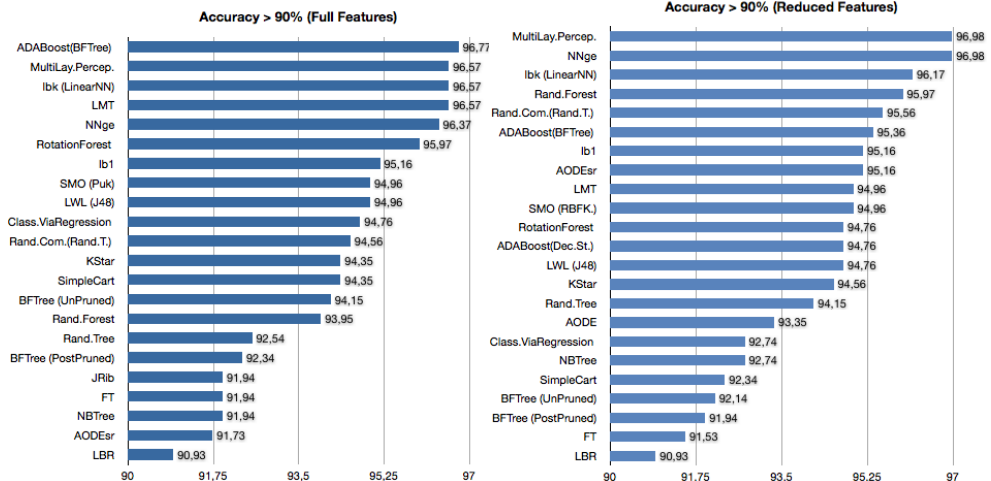
\includegraphics[width=\textwidth]{accuracy.png}
\caption{Preciznosti algoritama - sa svim atributima i bez}
\label{fig:acc}
\end{figure}

Na slici  \ref{fig:falsePos} se vidi isti trend kao i na slici  \ref{fig:acc}: smanjenjem broja atributa algoritmi zasnovani na stablima se lošije ponašaju dok algoritmi najbližih suseda i ``MultiLayerPerceptron'' daju bolje rezultate.

\begin{figure}[h!]
\centering
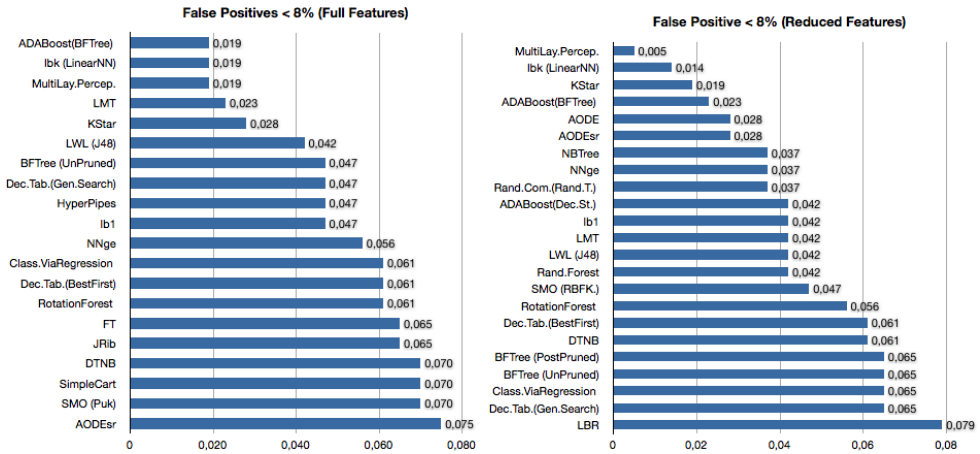
\includegraphics[width=\textwidth]{false_positive.png}
\caption{Lažno pozitivni - sa svim atributima i bez}
\label{fig:falsePos}
\end{figure}

Prema rezultatima dobijenim u  \cite{baca} vrlo je bitno da alat statičke analize ima malo lažno pozitivnih jer
u slučaju mnogo pogrešnih uzbuna programeri počinju da ignorišu te signale, ili još gore: kako bi izbegli upozorenja alata menjaju ispravan kod što dovodi do potencijalno
 novih greškaka. Na slici \ref{fig:falseNeg} se vidi da je ``NNge'' najbolji, što je i očekivano s obzirom na prilično
loše performanse što se tiče lažno pozitivnih.

\begin{figure}[h!]
\centering
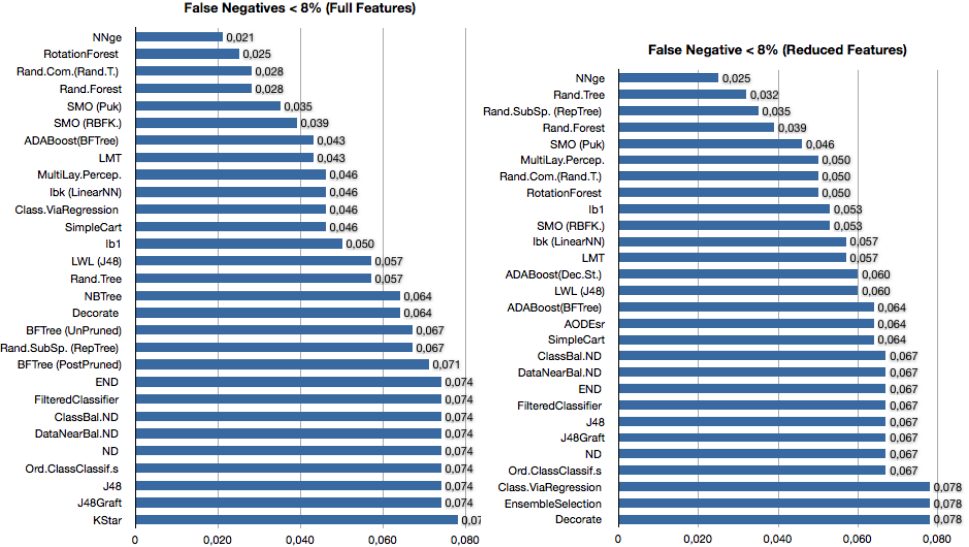
\includegraphics[width=\textwidth]{false_negative.png}
\caption{Lažno negativni - sa svim atributima i bez}
\label{fig:falseNeg}
\end{figure}



\subsection{Problem 2 - Luka}

Ovde pišem tekst.
Ovde pišem tekst.
Ovde pišem tekst.
Ovde pišem tekst.
Ovde pišem tekst.



\subsection{Problem 3 - Dimitrije}

Ovde pišem tekst.
Ovde pišem tekst.
Ovde pišem tekst.
Ovde pišem tekst.
Ovde pišem tekst.



\subsection{Problem 4 - Rastko}

Ovde pišem tekst.
Ovde pišem tekst.
Ovde pišem tekst.
Ovde pišem tekst.
Ovde pišem tekst.



% ==============================================================================
\section{Zaključak}
\label{sec:zakljucak}
% ==============================================================================



Ovde pišem zaključak.
Ovde pišem zaključak.
Ovde pišem zaključak.
Ovde pišem zaključak.
Ovde pišem zaključak.
Ovde pišem zaključak.
Ovde pišem zaključak.
Ovde pišem zaključak.
Ovde pišem zaključak.
Ovde pišem zaključak.
Ovde pišem zaključak.
Ovde pišem zaključak.



% ==============================================================================
\section{DELETE ME - help koji je bio na pocetku}
% ==============================================================================



\begin{primer}
	Problem zaustavljanja (eng.~{\em halting problem}) je neodlučiv \cite{haltingproblem}.
\end{primer}

\begin{primer}
	Za prevođenje programa napisanih u programskom jeziku C može se koristiti GCC kompajler \cite{gcc}.
\end{primer}

\begin{primer}
	Da bi se ispitivala ispravost softvera, najpre je potrebno precizno definisati njegovo ponašanje \cite{laski2009software}.
\end{primer}

Reference koje se koriste u ovom tekstu zadate su u datoteci {\em seminarski.bib}. Prevođenje u pdf format u Linux okruženju može se uraditi na sledeći način:
\begin{verbatim}
pdflatex TemaImePrezime.tex
bibtex TemaImePrezime.aux
pdflatex TemaImePrezime.tex
pdflatex TemaImePrezime.tex
\end{verbatim}
Prvo latexovanje je neophodno da bi se generisao {\em .aux} fajl. {\em bibtex} proizvodi odgovarajući {\em .bbl} fajl koji se koristi za generisanje literature.
Potrebna su dva prolaza (dva puta pdflatex) da bi se reference ubacile u tekst (tj da ne bi ostali znakovi pitanja umesto referenci). Dodavanjem novih referenci potrebno je ponoviti ceo postupak.


Broj naslova i podnaslova je proizvoljan. Neophodni su samo Uvod i Zaključak. Na poglavlja unutar teksta referisati se po potrebi.
\begin{primer}
	U odeljku \ref{sec:naslov1} precizirani su osnovni pojmovi, dok su zaključci dati u odeljku \ref{sec:zakljucak}.
\end{primer}

Još jednom da napomenem da nema razloga da pišete:
\begin{verbatim}
\v{s} i \v{c} i \'c ...
\end{verbatim}
Možete koristiti srpska slova
\begin{verbatim}
š i č i ć ...
\end{verbatim}


\addcontentsline{toc}{section}{Literatura}
\appendix
\bibliography{seminarski}
\bibliographystyle{plain}



\end{document}
